\label{ap:ap04}
\chapter{Estatística Aplicada I}
\section*{\textbf{A - ENUNCIADO}}
\subsection*{\textbf{1 Gráficos e tabelas}}


\begin{enumerate}[label=\alph*)]
\item \textbf{(15 pontos)} Elaborar os gráficos box-plot e histograma das variáveis “age” (idade da esposa) e “husage” (idade do
marido) e comparar os resultados
\item \textbf{(15 pontos)} Elaborar a tabela de frequencias das variáveis “age” (idade da esposa) e “husage” (idade do marido) e
comparar os resultados
\end{enumerate}

\subsection*{\textbf{2 Medidas de posição e dispersão}}

\begin{enumerate}[label=\alph*)]
\item \textbf{(15 pontos)} Calcular a média, mediana e moda das variáveis “age” (idade da esposa) e “husage” (idade do marido) e
comparar os resultados
\item \textbf{(15 pontos)} Calcular a variância, \ desvio padrão e coeficiente de variação das variáveis “age” (idade da esposa) e
“husage” (idade do marido) e comparar os resultados
\end{enumerate}



\subsection*{\textbf{3 Testes paramétricos ou não paramétricos}}

\begin{enumerate}[label=\alph*)]
\item \textbf{(40 pontos)} (40 pontos) Testar se as médias (se você escolher o teste paramétrico) \ ou as medianas (se você escolher o teste não
paramétrico) das variáveis “age” (idade da esposa) e “husage” (idade do marido) são iguais, construir os intervalos de
confiança e comparar os resultados.\\
\textbf{Obs: }
\begin{enumerate}[label=\textbf{\arabic*)}, font=\bfseries]
\item \textbf{Você deve fazer os testes necessários (e mostra-los no documento pdf) para saber se você deve usar o unpaired test
(paramétrico) ou o teste U de Mann-Whitney (não paramétrico), justifique sua resposta sobre a escolha.}
\item \textbf{Lembre-se de que os intervalos de confiança já são mostrados nos resultados dos testes citados no item 1 acima. }
\end{enumerate}
\end{enumerate}









%%%%%%%%%%%%%%%%%%%%%%%%%%%%%%%%%%%%%%%%%%%%%%%%%%%%%%%%%%%%%%%%%%%%%%%%%%%%%%%%%%%%%%%%%%%%%
\section*{\textbf{B - RESOLUÇÃO}}
\subsection*{\textbf{1 Gráficos e tabelas}}
\begin{adjustwidth}{1em}{}
\textbf{a) Elaborar os gráficos box-plot e histograma das variáveis “age” (idade da esposa) e “husage” (idade do
marido) e comparar os resultados}
\end{adjustwidth}

\begin{lstlisting}[language=R, style=input]
install.packages("car")
install.packages("fdth")
library(car)
library(fdth)

load("salarios.RData")

# Boxplots
Boxplot(salarios$age, data=salarios, id=list(method="y"), ylab="Idade das esposas")
Boxplot(salarios$husage, data=salarios, id=list(method="y"), ylab="Idade dos maridos")

# Histogramas
hist(salarios$age, breaks = 5, xlab="Idade das esposas", ylab = "Frequency")
hist(salarios$husage, breaks = 5, xlab="Idade dos maridos", ylab = "Frequency")
\end{lstlisting}
\begin{figure}[H]
\centering
\caption{Boxplot Idade das esposas}
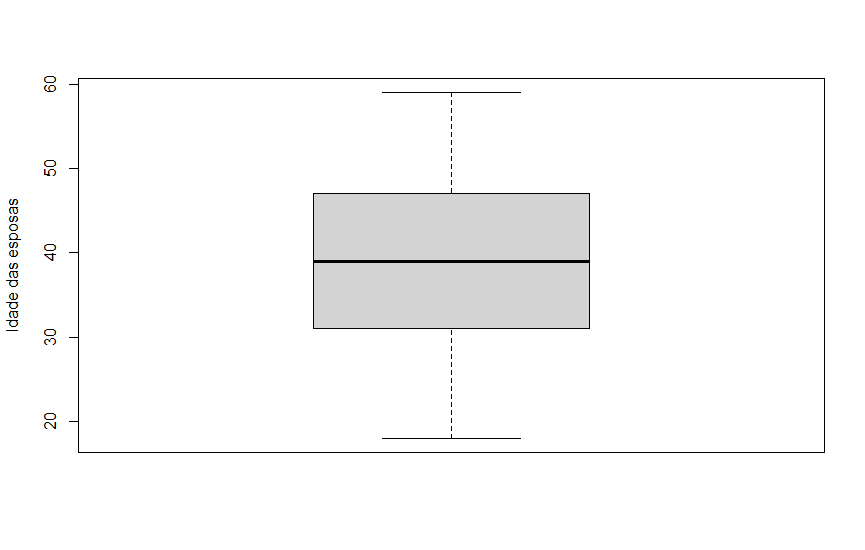
\includegraphics[width=1\linewidth]{apendices/fig/4_IAA004_1.png}
\caption*{Fonte: O autor (2025).}
\end{figure}
\begin{figure}[H]
\centering
\caption{Boxplot Idade das maridos}
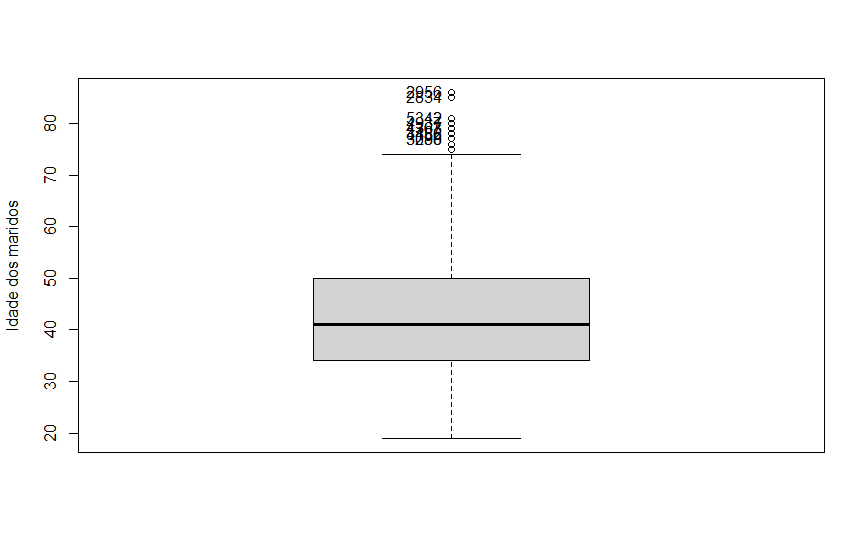
\includegraphics[width=1\linewidth]{apendices/fig/4_IAA004_2.png}
\caption*{Fonte: O autor (2025).}
\end{figure}
\begin{figure}[H]
\centering
\caption{Histograma Idade das esposas}
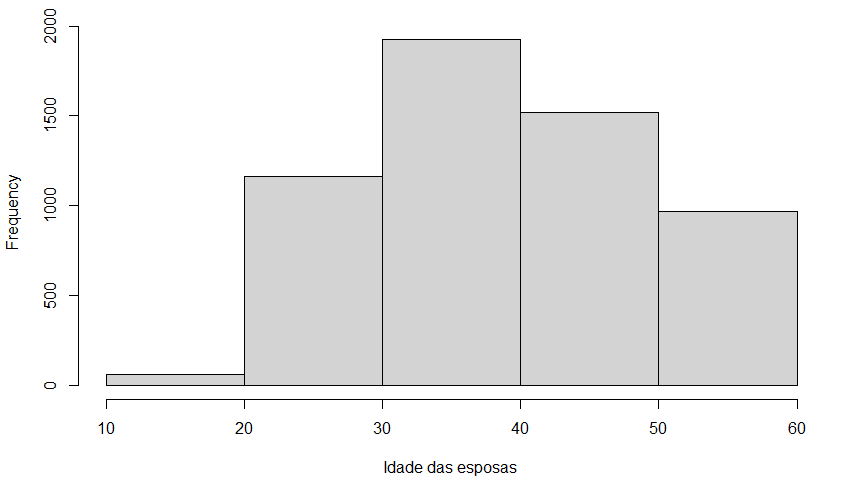
\includegraphics[width=1\linewidth]{apendices/fig/4_IAA004_3.png}
\caption*{Fonte: O autor (2025).}
\end{figure}
\begin{figure}[H]
\centering
\caption{Histogram Idade das maridos}
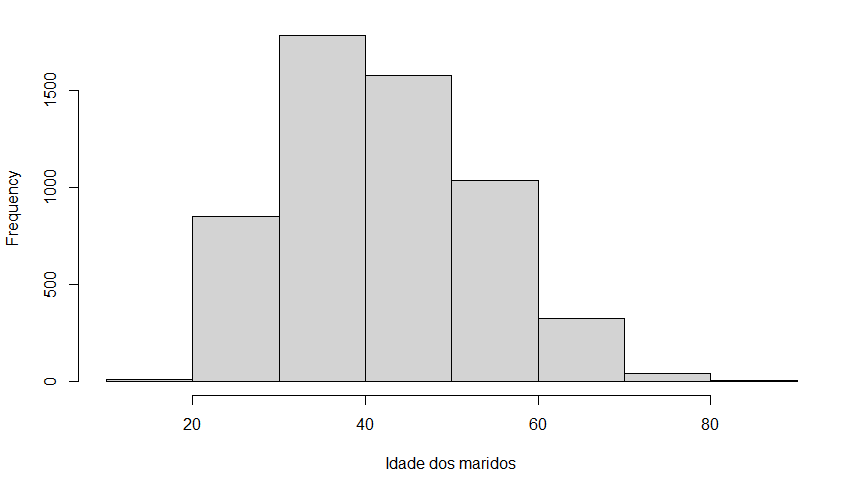
\includegraphics[width=1\linewidth]{apendices/fig/4_IAA004_4.png}
\caption*{Fonte: O autor (2025).}
\end{figure}

Analisando os gráficos box-plot podemos observar que as medianas das esposas e dos maridos parecem iguais, mas os limites superiores e inferiores diferem bastante, assim como a amplitude interquartílica. No caso o gráfico dos maridos possui o limite superior maior que as esposas além de possuir outliers. Já o gráfico das esposas tem maior amplitude interquartílica que o dos maridos.

Analisando os histogramas, observamos que há uma presença maior de esposas e maridos com idades entre 20 e 50 anos. À partir deste recorte a quantidade dos maridos cai drasticamente, porém, se alongando até acima de 80 anos. Já as mulheres, tem presença considerável até 60 anos e nenhum elemento acima desta idade. 

\begin{adjustwidth}{1em}{}
\textbf{b) Elaborar a tabela de frequencias das variáveis “age” (idade da esposa) e “husage” (idade do marido) e
comparar os resultados}
\end{adjustwidth}
\begin{lstlisting}[language=R, style=input] 
# TABELA DE FREQUENCIA DA VARIAVEL AGE (IDADE DA ESPOSA)
table_esposas <- fdt(salarios$age)
\end{lstlisting}
\begin{lstlisting}[language=R, style=output] 
    Class limits   f   rf rf(%)   cf  cf(%)
  [17.82,20.804)  61 0.01  1.08   61   1.08
 [20.804,23.787) 161 0.03  2.86  222   3.94
 [23.787,26.771) 312 0.06  5.54  534   9.48
 [26.771,29.754) 505 0.09  8.96 1039  18.44
 [29.754,32.738) 562 0.10  9.98 1601  28.42
 [32.738,35.721) 571 0.10 10.13 2172  38.55
 [35.721,38.705) 624 0.11 11.08 2796  49.63
 [38.705,41.689) 510 0.09  9.05 3306  58.68
 [41.689,44.672) 542 0.10  9.62 3848  68.30
 [44.672,47.656) 432 0.08  7.67 4280  75.97
 [47.656,50.639) 389 0.07  6.90 4669  82.87
 [50.639,53.623) 358 0.06  6.35 5027  89.23
 [53.623,56.606) 304 0.05  5.40 5331  94.62
  [56.606,59.59) 303 0.05  5.38 5634 100.00
\end{lstlisting}

\begin{lstlisting}[language=R, style=input] 
# TABELA DE FREQUENCIA DA VARIAVEL HUSAGE (IDADE DO MARIDO)
table_maridos <- fdt(salarios$husage)
\end{lstlisting}
\begin{lstlisting}[language=R, style=output] 
    Class limits   f   rf rf(%)   cf  cf(%)
  [18.81,23.671) 102 0.02  1.81  102   1.81
 [23.671,28.531) 466 0.08  8.27  568  10.08
 [28.531,33.392) 809 0.14 14.36 1377  24.44
 [33.392,38.253) 895 0.16 15.89 2272  40.33
 [38.253,43.114) 917 0.16 16.28 3189  56.60
 [43.114,47.974) 629 0.11 11.16 3818  67.77
 [47.974,52.835) 649 0.12 11.52 4467  79.29
 [52.835,57.696) 541 0.10  9.60 5008  88.89
 [57.696,62.556) 394 0.07  6.99 5402  95.88
 [62.556,67.417) 152 0.03  2.70 5554  98.58
 [67.417,72.278)  51 0.01  0.91 5605  99.49
 [72.278,77.139)  21 0.00  0.37 5626  99.86
 [77.139,81.999)   6 0.00  0.11 5632  99.96
  [81.999,86.86)   2 0.00  0.04 5634 100.00
\end{lstlisting}

Comparando as tabelas de frequência, podemos observar que as classes de frequências mais populosas para as esposas são de 29 a 35 anos e para os maridos de 33 a 43 anos. E a dispersão de idades é maior entre os maridos.


\subsection*{\textbf{2 Medidas de posição e dispersão}}

\begin{adjustwidth}{1em}{}
\textbf{a) Calcular a média, mediana e moda das variáveis “age” (idade da esposa) e “husage” (idade do marido) e
comparar os resultados}
\end{adjustwidth}
\begin{lstlisting}[language=R, style=input] 
# MEDIA
mean(salarios$age) # 39.42758
mean(salarios$husage) # 42.45296

((39.42758/42.45296)-1)*100 # -7.126429

# A media das idades das esposas eh de aproximadamente 
# 7% menor do que dos maridos.
\end{lstlisting}
\begin{lstlisting}[language=R, style=input] 
# MEDIANA
median(salarios$age) # 39
median(salarios$husage) # 41

((39/41)-1)*100 # -4.878049

# A mediana das idades das esposas eh de aproximadamente 
# 5% menor do que dos maridos.
\end{lstlisting}
\begin{lstlisting}[language=R, style=input] 
# MODA
table(salarios$age)
subset(table(salarios$age), 
    table(salarios$age) == max(table(salarios$age))) # 37

table(salarios$husage)
subset(table(salarios$husage), 
    table(salarios$husage) == max(table(salarios$husage))) # 44

# A moda da idade das esposa eh de 37 anos, com 217 pessoas.
# A moda da idade dos maridos eh de 44 anos, com 201 pessoas.

((37/44)-1)*100 # -15.90909
# A moda de idade das esposas eh aproximadamente 
# 16% menor do que dos maridos.
\end{lstlisting}

\begin{adjustwidth}{1em}{}
\textbf{b) Calcular a variância, \ desvio padrão e coeficiente de variação das variáveis “age” (idade da esposa) e
“husage” (idade do marido) e comparar os resultados}
\end{adjustwidth}
\begin{lstlisting}[language=R, style=input] 
# VARIANCIA
var(salarios$age)
var(salarios$husage)

# A variancia das idades das esposas eh 99.75234
# A variancia das idades dos maridos eh 126.0717

((99.75234/126.0717)-1)*100 # -20.8765

# A variancia das idades das esposas eh aproximadamente 
# 21% menor do que a variancia das idades dos maridos
\end{lstlisting}
\begin{lstlisting}[language=R, style=input] 
# DESVIO PADRAO
sd(salarios$age)
sd(salarios$husage)

# O desvio padrao das idades das esposas eh 9.98761
# O desvio padrao das idades dos maridos eh 11.22817

((9.98761/11.22817)-1)*100 # -11.04864

# O desvio padrao das idades das esposas eh aproximadamente 
# 11% menor que dos maridos
\end{lstlisting}
\begin{lstlisting}[language=R, style=input] 
# COEFICIENTE DE VARIACAO DAS VARIAVEIS
meanE <- mean(salarios$age)
meanM <- mean(salarios$husage)

sdE <- sd(salarios$age)
sdM <- sd(salarios$husage)

cvM <- (sdM/meanM)*100 # 26.44849
cvM
cvE <- (sdE/meanE)*100 # 25.33153
cvE

# O coeficiente de variacao do rendimento das esposas 
# eh de aproximadamente 26% e dos maridos eh de 
# aproximadamente 25%. 
# Ambos possuem dispersao media.
\end{lstlisting}


\subsection*{\textbf{3 Testes paramétricos ou não paramétricos}}

\begin{adjustwidth}{1em}{}
\textbf{a) Testar se as médias (se você escolher o teste paramétrico) \ ou as medianas (se você escolher o teste não
paramétrico) das variáveis “age” (idade da esposa) e “husage” (idade do marido) são iguais, construir os intervalos de
confiança e comparar os resultados.}
\end{adjustwidth}

Checagens preliminares para verificar as exigências do teste: 1) Amostras independentes, 2) normalidade e 3) homogeneidade das variâncias entre grupos 4) outliers


\begin{enumerate}
    \item[1)] Amostras independentes: Sim, pois os grupos de esposas e maridos provêm de indivíduos distintos.
\end{enumerate}

\begin{enumerate}
    \item[2)] Normalidade: Não, utilizando a regra de bolso, como o p-value eh inferior a 0.05, a variavel ``idade'' NÃO é normalmente distribuída .
\end{enumerate}
\begin{lstlisting}[language=R, style=input] 
    # Executanto teste de normalidade de Kolmogorov-Smirnov
    lillie.test(idades$idade)  
    # p-value = 0.00000000000000022
\end{lstlisting}

\begin{enumerate}
    \item[3)] Homogeneidade das variâncias: Não. Conforme observa-se no teste abaixo, o valor da estatística F calculada é 0.79123. Como esse valor se encontra na região de rejeição de H0, então rejeitamos a hipótese de que as variâncias são estatisticamente iguais. 
\end{enumerate}
\begin{lstlisting}[language=R, style=input] 
     # Vamos usar o teste F com as seguintes hipoteses:
    
    # H0: As variancias sao estatisticamente iguais(homogeneas)
    # HA: As variancias nao sao estatisticamente iguais(homogeneas)
    
    # Executando o teste F 
    res.ftest <- var.test(idade ~ group, data = idades)
    res.ftest
    
    # Obtendo o valor tabelado da distribuicao F
    qf(0.95, 5633, 5633)
    # temos F=1,04
    # para a outra cauda temos:
    1/1.04
    # F = 0,96
    
    # Vamos construir o grafico:
    dist_f(f = 1.04, deg.f1 = 5633, deg.f2 = 5633)
    dist_f(f = 0.96, deg.f1 = 5633, deg.f2 = 5633)  
\end{lstlisting}

\begin{figure}[H]
\centering
\caption{Gráfico da distribuição F}
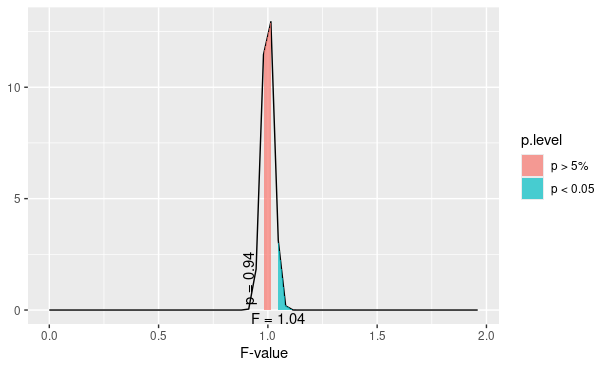
\includegraphics[width=.9\textwidth]{apendices/fig/4_IAA004_5.png} 
\caption*{Fonte: O autor (2025).}
\label{fig:subim1}
\end{figure}

\begin{enumerate}
    \item[4)] Outliers: Sim. Ao observar o boxplot dos maridos percebe-se alguns outliers.
\end{enumerate}

Dada as checagens anteriores de que a distribuição da variável idade NÃO é normalmente distribuída, as variâncias não serem estatisticamente iguais e também haverem outliers, não podemos usar um teste paramétrico para testar os dados, portanto utilizaremos o teste não paramétrico Mann Whitney U Test.

Queremos saber se a idade mediana das esposas difere da idade mediana dos maridos. Portanto, testando se a idade mediana dos maridos é igual a idade mediana das esposas temos as seguintes hipóteses:

\begin{itemize}
\item  H0: A idade mediana dos maridos é estatisticamente igual a idade mediana das esposas
\item  Ha: A idade mediana dos maridos não é estatisticamente igual a idade mediana das esposas\hfill \break
\end{itemize}

\begin{lstlisting}[language=R, style=input] 
    # Executando o teste Mann Whitney U Test
    res <- wilcox.test(idade ~ group, data = idades,
                       exact = FALSE, conf.int=TRUE)
    res    
\end{lstlisting}
\begin{lstlisting}[language=R, style=output] 
	Wilcoxon rank sum test with continuity correction

data:  idade by group
W = 13619912, p-value < 0.00000000000000022
alternative hypothesis: true location shift is not equal to 0
95 percent confidence interval:
 -3.000024 -2.000033
sample estimates:
difference in location 
             -2.999966 
\end{lstlisting}
O p-value do teste eh 0.00000000000000022, que eh menor que o nivel de significancia 0,05. Podemos concluir que a idade mediana dos maridos é estatisticamente diferente da idade mediana das esposas (rejeitamos H0). O intervalo de confianca da diferenca entre as medianas esta entre 3.000024 e 2.000033, com uma mediana de 2.999966. 